\chapter{Introdução}


O desenvolvimento de software normalmente encontra problemas relacionados ao cumprimento dos prazos de entrega. Tal situação pode ocorrer devido, a exemplo do aumento de demandas extras, desvios nos requisitos e problemas internos na equipe. Assim, a solução para atrasos de entrega pode estar em soluluções específicas, entretanto, existem elementos universais que podem mitigar ou combater esse problema, como o reuso de software. Este trabalho de conclusão de curso busca padronizar o controle de acesso dos softwares, abastraindo-o e tornando-o passível de maior reuso como um serviço reutilizável no desenvolvimento de software, reduzindo assim o tempo de desenvolvimento e manutenção.


\section{Motivação}


Otimizar o desenvolvimento de software é uma tarefa árdua e bastante estudada. A área de Engenharia de Software estuda maneiras de melhorar o desenvolvimento de software mediante processos e práticas de desenvolvimento. Qualquer melhoria durante a construção de um sistema, normalmente acaba por prover uma economia no orçamento de desenvolvimento e/ou manutenção. Assim, é possível inferir que melhorias no processo de desenvolvimento de sistemas, pode satisfazer as necessidades desde o programador, com um trabalho facilitado, até o cliente final com redução de custo.


\section{Problema} %começar de forma mais genérica


O impacto dessa má prática atinge fortemente a manutenibilidade do software, grande transtorno diante de uma alteração que poderia ser simples caso. A abordagem do reuso pode inclusive, abranger mais de um projeto numa organização, fazendo que até mesmo módulos inteiros sejam reaproveitados. 


\section{Objetivos}


\begin{itemize}
	\item Objetivo geral: Seguindo a boa prática de projetar o software, o objetivo geral deste trabalho é prover o reuso de código, utilizando padões que mantenham o componente de código na melhor forma possível para ser acoplado em outros softwares sem muitas dificuldades adicionais.
	\item Objetivo específico: O controle de acesso de um sistema, já que o mesmo está presente sem remodelações significativas nos sistemas de uma organização. Assim, o objetivo é desenvolver tal módulo como um serviço, deixando-o isolado e gerando a possibilidade de qualquer sistema consumir tal módulo como um serviço. Dessa forma, ao projetar um novo software para uma organização por exemplo, ao invés de incluir o módulo de controle de acesso, projetaria-se o código para consumir o serviço de contrle de acesso que seria um projeto à parte. Ele também apresenta a vantagem de ter interoperabilidade entre linguagens de programação, já que realiza a comunicação através de JSON, seguindo padrões atuais. Assim, tem-se uma constância no módulo de acesso independentemente da possível necessidade de migração de tecnologia.
\end{itemize}


\section{Metodologia}
%<como será feito, como resolver o problema apontado inicialmente>

A fim de selecionar as tecnologias a serem utilizadas na implementação deste trabalho, nesta seção as mesmas serão apresentadas com base nas indústria de desenvolvimento de software. (estado da prática). Para embasar esse cenário, serão exibidas estatísticas que refletem a situação do mercado.

%<analise de literatura | design | implementação | validação>
Baseando-se nas tecnologias no cenário atual do desenvolvimento, dispomos de algumas opções eficientes para a implementação da solução. Dentre as possibilidades, considerando a facilidade para futura manutenção e continuidade do projeto, tende-se a optar por uma tecnologia popular. A linguagem de programação adotada é PHP. A escolha é fundamentada na pesquisa da RedMonk de 2015 \cite{Grafico-RedMonk} , que evidencia o uso das linguagens de programação de acordo com as discussões no StackOverflow e repositórios no GitHub. É possível constatar a popularidade do PHP no cenário atual apresentado em \ref{fig:graficoRedmonk}, na qual o PHP é apresentado na terceira colocação, apenas atrás do lider JavaScript e do segundo colocado, o Java.


\begin{figure}
	\label{fig:graficoRedmonk}
	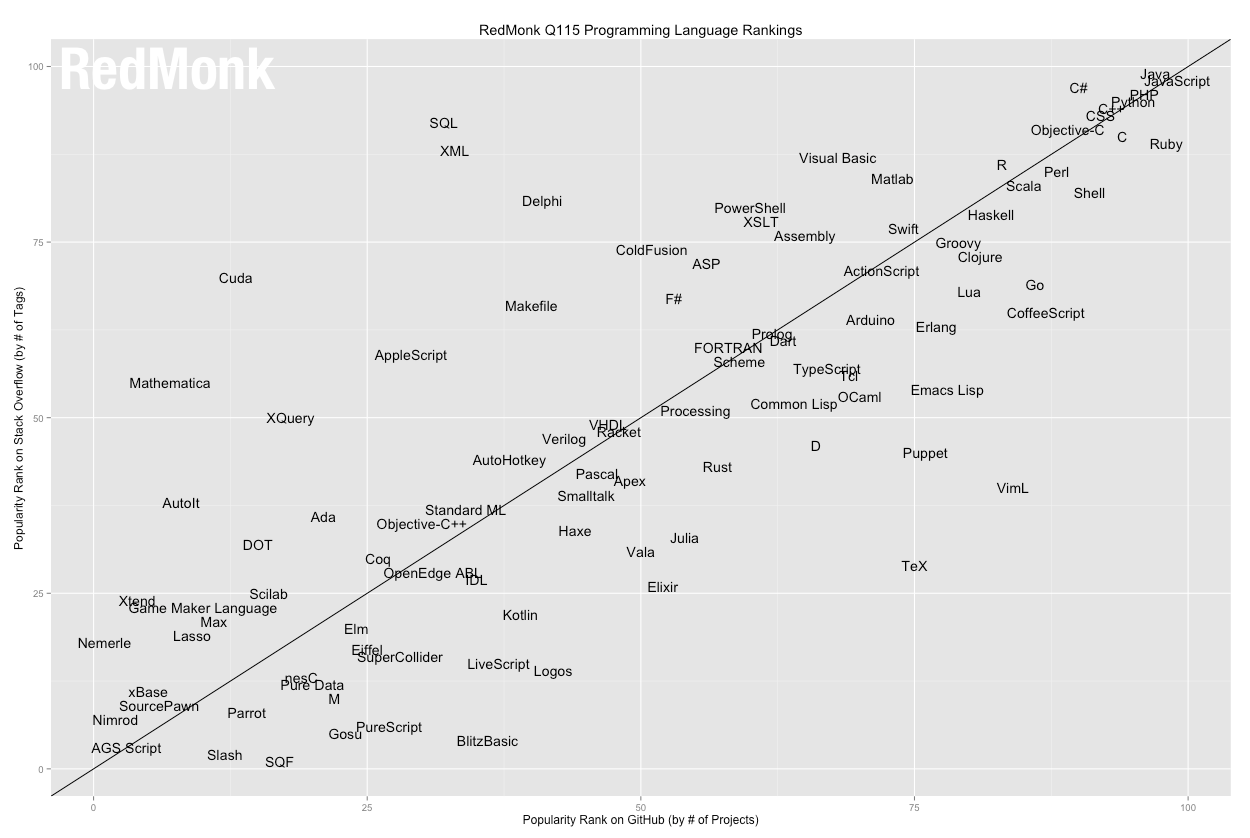
\includegraphics[width=1\textwidth]{img/grafico_redmonk}
	\caption{Ranking das liguagens de programação no Stack Overflow e Github}
\end{figure}


Entretanto, não seria inteligente desenvolver um sistema completo sem o auxílio de um framework. Dentre os frameworks disponíveis para PHP, hoje o destaque está com o Laravel, que se encontra no topo dentre os mais utilizados no momento. 
 

A WebHostFace, uma empresa de hospedagem, compilou várias estatísticas para criar um infográfico mostrando os frameworks PHP mais populares de 2015. Utilizando informações sobre os próprios clientes, o Google Trends, estatísticas de repositórios do GitHub e a pesquisa do SitePoint “Best PHP Frameworks 2015”, a WebHostFace elaborou o gráfico \ref{fig:graficoWebhostface}. %O gráfico está sendo mostrado no local errado apesar da ordem


\begin{figure}
	\label{fig:graficoWebhostface}
	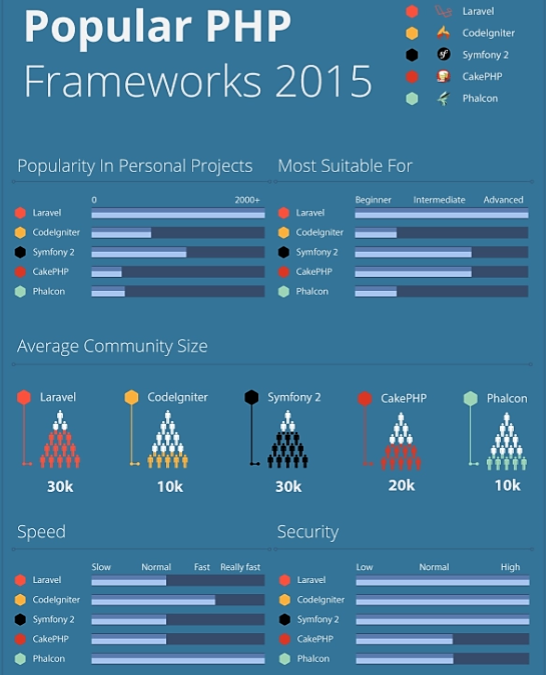
\includegraphics[width=1\textwidth]{img/infografico_webhostface}
	\caption{Infográfico da WebhostFace, exibindo a popularidade dos Frameworks PHP em 2015}
\end{figure}


Como pode ser verificado no gráfico \ref{fig:graficoWebhostface}, tem-se a evidência que o Laravel em 2015 teve a maior popularidade em projetos pessoais e tem a maior comunidade entre os concorrentes, o que o torna uma boa escolha para a escrita de um software que será continuado por terceiros.


Para elaborar os recursos de interface e integrar ao back-end PHP do sistema, será adotado o já conhecido AngularJS, ferramenta sólida e conhecida no aspecto em questão. 


Dados coletados via Google Trends em, que propõe comparações entre termos pesquisados, revela a popularidade do AngularJS diante de alguns dos principais concorrentes. O gráfico \ref{fig:graficoGoogleTrendsFerramentasFront} evidencia o cenário.


\begin{figure} % \ref{fig:graficoGoogleTrendsFerramentasFront}. 
	\label{fig:graficoGoogleTrendsFerramentasFront}
	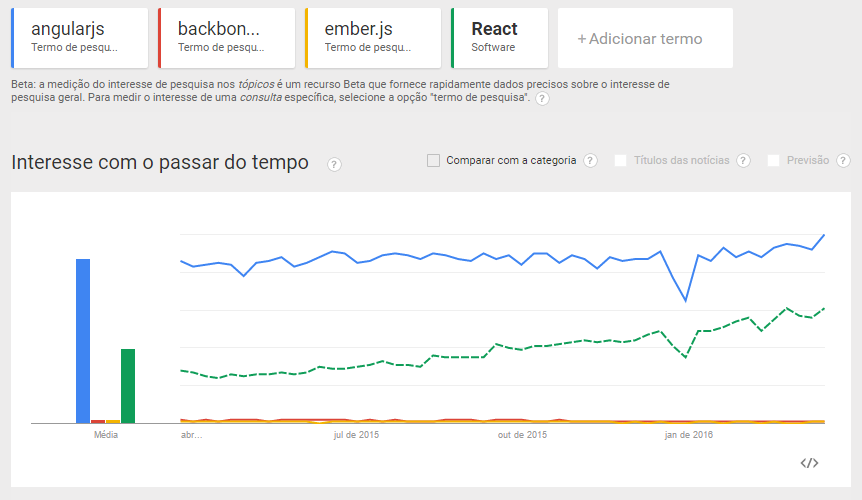
\includegraphics[width=1\textwidth]{img/grafico_ferramentas_front}
	\caption{Gráfico do Google Trends exibindo as pesquisas por ferramentas front-end}
\end{figure}


\section{Resultados Esperados}


Realizando o uso do proposto módulo de controle de acesso como serviço, espera-se que ocorram os seguintes ganhos:


\begin{itemize}
	\item Servir a projetos de diferentes liguagens.
	\item Atender a projetos de diferentes plataformas (Web, Desktop, Mobile).
	\item Facilidade de configuração das permissões.
	\item Extinção do módulo de permissões nos projetos em que o trabalho proposto será aplicado.
\end{itemize}


\section{Fora de Escopo}


Diante da possibilidade de gerência dos sistemas, módulos e funcionalidades contratadas, seria possível estender o sistema aqui proposto, complementando-o com uma abordagem financeira, controlando o acesso do cliente mediante o pagamento do que está contratado pelo cliente. Também existe a possibilidade de realizar o controle por número de usuários que estão logados no sistema contratado ou por módulo, mediante uma evolução na implementação. Uma possível solução para a última situação seria o sistema consumidor enviar uma notificação (post) ao sistema de gerenciamento de módulo num determinado intervalo de tempo, o usuário logado no sistema. O sistema de gerenciamento de módulos responderia internamente à sinalização, mantendo registro de usuário ativo. Caso o usuário final saia do sistema, enviaria o sinal de logout e caso fechasse o navegador, a sessão seria encerrada por tempo de inatividade (falta de envio da notificação de uso).


\section{Estrutura do Trabalho} %<breve resumo sobre os capítulos do TCC>


Neste tópico, tem-se uma breve apresentação dos capítulos que compõem este trabalho de conclusão de curso:

\begin{itemize}
	\item Capítulo 1: Referencial teórico, fundamentando os principais conceitos que compõem os elementos marcantes do trabalho.
	\item Capítulo 2: Introdução, apresentando uma visão geral do trabalho.
	\item Capítulo 3: Proposta, contendo o detalhamento do trabalho proposto, baseando-se nos aterfatos da engenharia de software.
	\item Capítulo 4: Análise
	\item Capítulo 5: Conclusão
\end{itemize}

